\section{Итератори}

\begin{frame}{Преглед}
\begin{center}
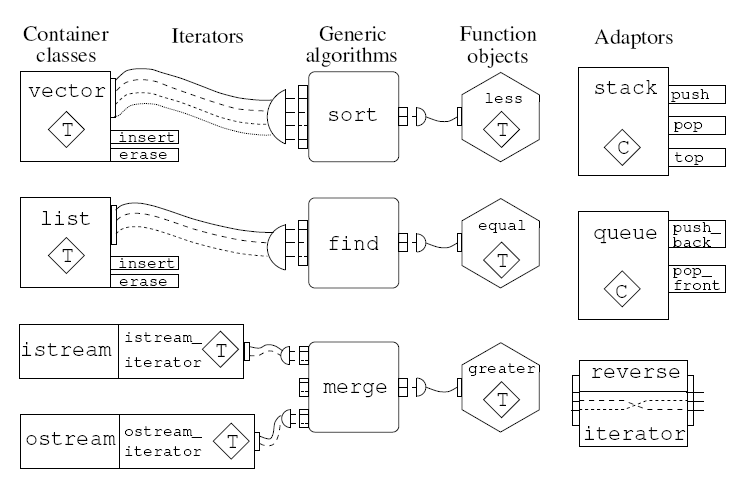
\includegraphics[width=\textwidth]{images/iterators}
\end{center}
\end{frame}

\begin{frame}{Што се итератори?}
\begin{itemize}
\item Објекти налик на покажувачи кои се користат во алгоритамските функции за
изминување на секвенца од објекти  
\item Медијатор, посредник помеѓу контејнерите и генеричките алгоритми
\item Независност во креирањето на алгоритмите и конејнерите
\end{itemize}
\end{frame}

\begin{frame}{Класификација на итераторите}
\begin{itemize}
\item Input  
\item Output
\item Forward
\item Bidirectional
\item Random access
\end{itemize}
\end{frame}

\begin{frame}{Опсег на итераторите}
\begin{itemize}
\item \texttt{[first, last)}  
\item Operator \texttt{++}
\item Empty range: \texttt{first == last}
\end{itemize}
\end{frame}

\begin{frame}[fragile]{Input iterators}
\begin{block}{Пример}
\begin{lstlisting}
template<typename InputIterator, typename T>
InputIterator  find(InputIterator first, InputIterator last, const T& value) {
    while(first != last && *first != value)
        ++first;
    return first;
}
\end{lstlisting}
\end{block}
За да find работи коректно, потребно е дефинирање на:
\begin{lstlisting}
first != last
++first
*first
\end{lstlisting}
\end{frame}

\begin{frame}{Input iterators}
\begin{itemize}
  \item Во рамките на \texttt{input} итераторот е дефинирана операцијата ==, за
  тестирање на еднаквост
  \item Дефиниран е и операторот \texttt{Postfix ++}, кој ја враќа вредноста која ја имал
  итераторот пред да биде инкрементиран
  \item Операцијата \texttt{*first = ..}, не мора да е подржана од
  \texttt{input} итераторите
  \item Терминот \texttt{input iterator} не се однесува на конкретен податочен тип, туку
  на фамилија од типови кои ги задоволуваат барањата
\end{itemize}
\end{frame}

\begin{frame}[fragile]{Output iterators}
\begin{itemize}
  \item Овој тип на итератори дозволуваат да запишуваме вредности во секвенца,
  но не гарантираат дека може од истата да читаме
  \item \texttt{*first = \ldots}, е во ред
  \item Додека \texttt{*first} не може да се користи во изрази за да ја добиеме неговата
  вредност
  \item Нема потреба од дефинирање на == и !=
  \item Операторите ++ се дефинирани
\end{itemize} 

\begin{block}{Пример}
\begin{lstlisting}
template<typename InputIterator, typename OutputIterator>
void copy(InputIterator first, InputIterator last, OutputIterator result) {
    while(first != last){
        *result = *first;
        ++first;
        ++result;
    }
}
\end{lstlisting}
\end{block}
\end{frame}

\begin{frame}[fragile]{Forward iterators}
\begin{itemize}
  \item Итератор кој овозможува читање и запишување
  \item Изминувањето на елементите е возможно само во една насока
\end{itemize}
\begin{block}{Пример}
\begin{lstlisting}
template<typename ForwardIterator, typename T>
void replace(ForwardIterator first, ForwardIterator last, const T& x, const T& y){
    while(first != last){
        if (*result ==x)
        *first = y;
        ++first;
    }
} 
\end{lstlisting}
\end{block}
\end{frame}

\begin{frame}[fragile]{Forward iterators}
\begin{block}{Пример}
\begin{lstlisting}
deque<char> d;
replace(d.begin(), d.end(), 'e', 'o');
\end{lstlisting}
\end{block}
Претходните наредби се возможни поради фактот што \texttt{deque<T>::iterator} ги
задоволува сите барања на \texttt{forward iterator}
\end{frame}


\begin{frame}[fragile]{Bidirectional Iterators}
\begin{itemize}
  \item Итератори кои овозможуваат изминување во двете насоки
  \item Имплементација на сите својства на forward итераторите, дополнително
  имплементација и на \texttt{++/--} операторите во двете верзии (постфикс и суфикс)
\end{itemize}
\begin{block}{Пример}
\begin{lstlisting}
list<int> l;
revers(l.begin(), l.end());
\end{lstlisting}
\end{block}
Претходните наредби се возможни поради фактот што \texttt{list<T>::iterator} ги
задоволува сите барања на \texttt{bidirectional} итераторите
\end{frame}

\begin{frame}[fragile]{Random Access Iterators}
\begin{itemize}
  \item Директен пристап до било кој елемент во секвенцата
  \item \texttt{binary\_search(first, last, value)}
  \item \texttt{O(logN) < O(N)}
\end{itemize}
\begin{block}{Пример}
\begin{lstlisting}
vector<int> v;
bool found = binary_search(v.begin(), v.end(), 5);
\end{lstlisting}
\end{block}
\begin{itemize}
\item \texttt{Random Access} итераторите ги подржуваат сите операции на \texttt{bidirectional}
итераторите дополнети со
\item \texttt{r+n, r-n}
\item \texttt{r[n], *(r+n)}
\item \texttt{r+=n, r-=n}
\item \texttf{r-s} (одземање на итератори)
\item \texttt{r<s, r>s, r<=s, r>=s}
\end{itemize}
\end{frame}

\begin{frame}[fragile]{Insert iterators}
\begin{itemize}
  \item Вметнување на елемент на одредена позиција со помош на функциите за
  вметнување на елементи дефинирани во контејнерот 
  \item \texttt{back\_insert\_iterator<Container>}, ја користи
  \texttt{push\_back} функцијата
  \item \texttt{front\_insert\_iterator<Container>}, ја користи
  \texttt{push\_front} функцијата
  \item \texttt{insert\_iterator<Container>}, ја користи \texttt{insert}
  функцијата на содветната контејнер класа
\end{itemize}
\end{frame}

\begin{frame}[fragile]{Insert iterators}{Пример}
\begin{lstlisting}
vector<int> v;
deque<int> d(200,1);
copy(d.begin(), d.end(), v.begin()); // error
copy(d.begin(), d.end(), back_insert_iterator<vector<int> >(v));
\end{lstlisting}
За полесно користење на \texttt{back\_insert\_iteratorot}, во STL е дефинирана
генеричка темплејт функција \texttt{back\_insert}. 
\begin{lstlisting}
template <typename Container>
inline back_insert_iterator<Container> 
back_insert(Container& x) {
   return back_insert_iterator<Container> (x);
}
\end{lstlisting}
\texttt{vector}, \texttt{list} и \texttt{deque} (бидејќи содржат \texttt{push\_back} функција)
\texttt{front\_insert\_iterator} - \texttt{deque}, \texttt{list} контејнери кои
имаат дефинирано \texttt{push\_front} функција
\end{frame}

\begin{frame}[fragile]{Insert iterator}
Функција која може да се примени на било кој контејнер, бидејќи сите контејнери
обезбедуваат \texttt{insert(iterator, value)} функција 
\begin{lstlisting}
copy(&array[0], &array[100], inserter(deque1, deque1.begin() + 1));
\end{lstlisting}
\begin{block}{Пример \texttt{istream\_iterator, ostream\_iterator}}
\texttt{istream\_iterator<T>()}, \texttt{input} итератор кој се однесува како
маркер кој го означува краjот на \texttt{istream}-от
\begin{lstlisting}
merge(v.begin(), v.end(), istream_iterator<int>(cin), istream_iterator<int>(), back_inserter(l));
merge(istream_iterator<int>(cin), istream_iterator<int>(), v.begin(), v.end(),  back_inserter(l));
\end{lstlisting}
\end{block}
\end{frame}

\begin{frame}[fragile]{Ostream iterators}
Овој тип на итератор не дозволува читање на вредноста кон која референцира истиот
\begin{block}{Пример}
\begin{lstlisting}
list<int> list1
ostream_iterator<int> out(cout, "\n");
copy(list1.begin(), list1.end(), out);
merge(v.begin(), v.end(), l.begin(), l.end(), ostream_iterator<int>(cout," "));
\end{lstlisting}
\end{block}

\end{frame}

\begin{frame}{Преглед на итераторите}
\begin{center}
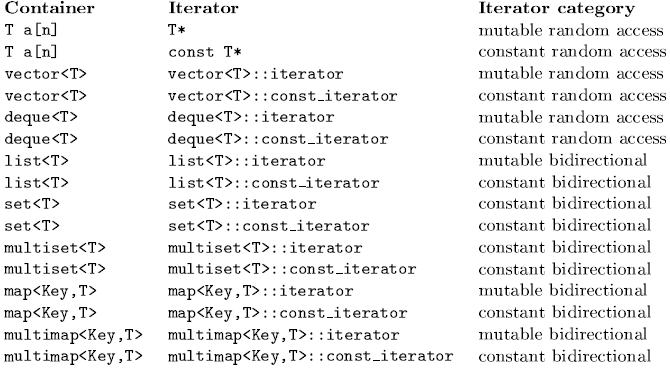
\includegraphics[width=\textwidth]{images/overview}
\end{center}
\end{frame}

\section{Алгоритми}

\begin{frame}{Алгоритми}
\begin{itemize}
  \item Некои операции се карактеристични и специфични само за контејнерите,
  обезбедени како дел од нивната имплементација и дефиниција
  \item Генеричките алгоритми се заеднички за сите контејнери
  \item \texttt{\#include <algorithm>}
  \item Header фајлот вклучува и некои додатни (помошни) функции \texttt{min()}, \texttt{max()} и
  \texttt{swap()}.
  \item Некои STL алгоритми се користат за нумеричко процесирање. Поради тоа тие
  се дефинирани во \texttt{<numeric>} хедер фајлот
  \item Кога користиме алгоритми, често ни се потребни функциски објекти и
  функциски адаптери. Тие се дефинирани во \texttt{<functional>} хедер фајлот.
\end{itemize}
\end{frame}

\begin{frame}{Класификација на алгоритмите}
\begin{itemize}
  \item Алгоритми кои оперираат само како \texttt{read only}
  \item Алгоритми кои ги модифицираат елементи
  \item Алгоритми кои го менувата редоследот на елементите
  \item Името на алгоритмот ни дава јасна слика за неговата нaмена
  \item Дизајнерите на STL вклучуваат два специфични суфикса за распознавање на алгоритмите
\end{itemize}
\end{frame}

\begin{frame}{\texttt{\_if} суфикс}
 Се користи кога може да повикаме две форми на алгоритам
кој има ист број на параметри. Верзијата без суфиксот се користи за вредност, а
верзијата со \texttt{\_if} суфиксот се користи за функции и функциски објекти.
\begin{block}{Пример}
\texttt{find()} бара елемент кој има одредена вредност\\
\texttt{find\_if()} бара елемент кој запознава одреден критериум претставен со
функциски објект
\end{block}
\end{frame}

\begin{frame}{\texttt{\_copy} суфикс}
 Се користи за да се нагласи дека освен тоа што можеме да манипулираме со
 елемнтите исто така можеме да ги копираме во дестинационен опсег.
\begin{block}{Пример}
\texttt{reverse()} го превртува редот на елементите внатре во дадениот опсег\\
\texttt{reverse\_copy()} ги копира елементите во друг опсег во обратен редослед.
\end{block}
\end{frame}

\begin{frame}{Класификација на алгоритмите}
\begin{itemize}
  \item Немодифицирачки алгоритми(Non modifying algorithms)
  \item Модифицирачки алгоритми (Modifying algorithms)
  \item Отстранувачки алгоритми (Removing algorithms)
  \item Менувачки алгоритми (Mutating algorithms) 
  \item Сортирачки алгоритми (Sorting algorithms) 
  \item Сортирачки ранг алгоритми (Sorted range algorithms)
  \item Нумерички алгоритми (Numeric algorithms)
\end{itemize}
\end{frame}

\begin{frame}{Немодифицирачки алгоритми}
Овие алгоритми не го менуваат ни редот ни вредноста на елементите кои ги
процесираат. Тие оперираат со влезните и предните(forward) итераторите, затоа
можеме да ги повикуваме за сите стандардни контејнери.
\end{frame}

\begin{frame}{Немодифицирачки алгоритми}
\begin{center}
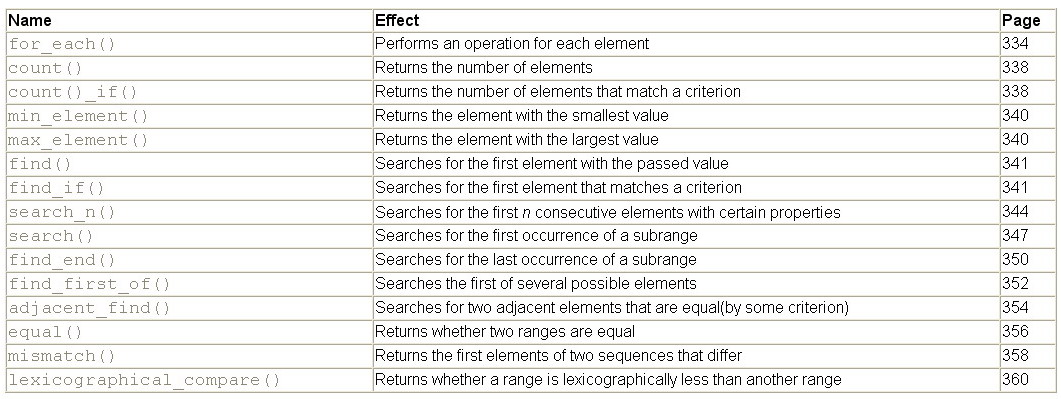
\includegraphics[width=\textwidth]{images/non_modifying}
\end{center}
\end{frame}

\begin{frame}{Модифицирачки алгоритми}
Модифицирачките алгоритми ја менуваат вредноста на елементите. Тие може да ги
модифицираат елементите директно во зададениот опсег или да ги модифицираат
додека се копираат во друг опсег. Ако елементите се копираат во дестинационен
опсег, изворишниот опсег не се менува.
\end{frame}

\begin{frame}{Модифицирачки алгоритми}
\begin{center}
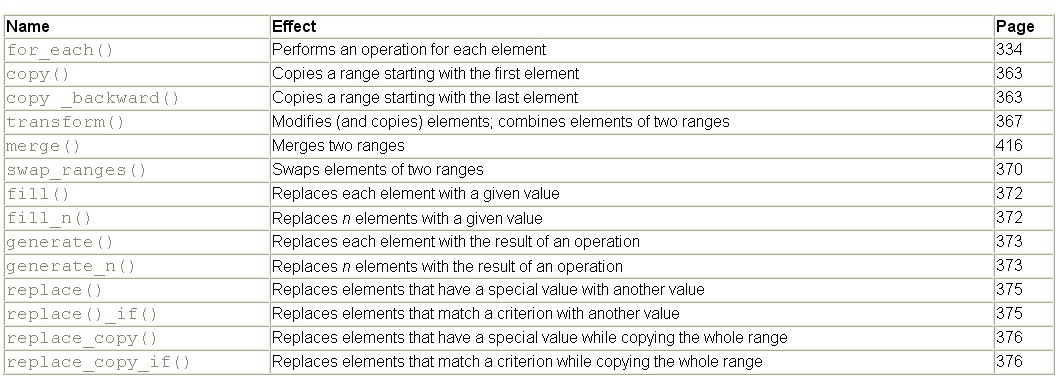
\includegraphics[width=\textwidth]{images/modifying}
\end{center}
\end{frame}

\begin{frame}{Модифицирачки алгоритми}
\begin{itemize}
  \item \texttt{for\_each()} директно ги модифицира влезните аргументи,
  аргументите мора да бидат проследени по референца
  \item transform() користи операции кои го враќаат модифицираниот аргумент,
  може да се користи за да го додели резултатот на оригиналниот
  \item Пристапот на transform() е малку поспор бидејќи враќа и го назначува
  (assigns) резултатот наместо да го модифицира елементот директно
\end{itemize}
\end{frame}
 
\begin{frame}{Отстранувачки алгоритми}
\begin{itemize}
  \item Отстранувачките алгоритми се специјална форма на модифицирачки
  алгоритми. 
  \item Тие може да острануваат елементи или во единчен опсег или додека се
  копираат во друг опсег.
  \item Кога користиме modifying algorithms, не можеме да користиме асоцијативни
  контејнери како дестинација бидејќи елементите на асоцијативните контејнери се сметаат за константи.
  \item Мораме да забележиме дека removing algorithms ги отстрануваат елементите
  само со нивно препишување (by overwriting) со следните елементи кои не се
  отстранети. Поради тоа, тие не го менуваат бројот на елементите во опсегот во
  кој оперираат. Наместо тоа, тие ја враќаат позицијата на новиот „крај“ на
  рангот
\end{itemize}
\end{frame}

\begin{frame}{Отстранувачки алгоритми}
\begin{center}
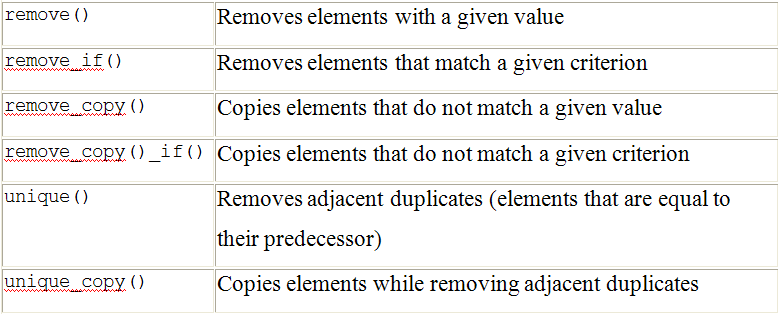
\includegraphics[width=\textwidth]{images/removing}
\end{center}
\end{frame}

\begin{frame}{Mutating Algorithms}
\begin{itemize}
  \item Mutating algorithms се алгоритми кои го менуваат редот на елементите (не
  нивните вредности) со назначување (доделување) и менување (by assigning and
  swapping) на нивните вредности.
  \item Како и кај modifying алгоритмите, и овде неможеме да користиме асоцијативни
  контејнери како дестинација бидејќи елементите на асоцијативниот контејнер се константи.
\end{itemize}
\end{frame}

\begin{frame}{Mutating Algorithms}
\begin{center}
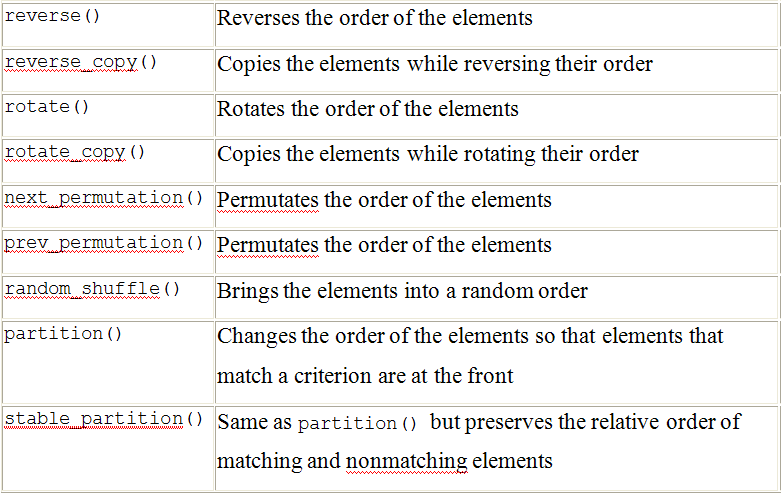
\includegraphics[width=\textwidth]{images/mutating}
\end{center}
\end{frame}

\begin{frame}{Сортирачки алгоритми}
\begin{itemize}
  \item Сортирачките алгоримти се специјален вид на mutating алгоритми бидејќи
  тие исто така го менуваат редот на елементите.
  \item Сепак, сортирањето е покомплицирано и затоа обично зема повеќе време
  отколку едноставнати менувачи (mutating) операции.
  \item Имаат потреба, односно бараат \texttt{random access iterators} (за
  дестинацијата).
\end{itemize}
\end{frame}
 

\begin{frame}{Сортирачки алгоритми}
\begin{center}
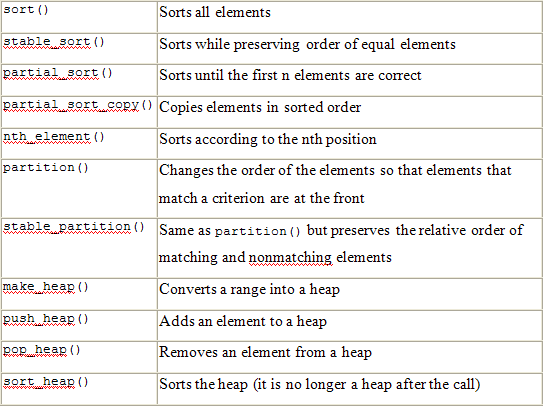
\includegraphics[width=0.8\textwidth]{images/sorting}
\end{center}
\end{frame}

\begin{frame}{Numeric и Heap алгоритми}
\begin{itemize}
  \item \texttt{accumulate}
  \item \texttt{inner\_product}
  \item \texttt{adjcent\_difference}
  \item \texttt{partial\_sum}
  \item \texttt{make\_heap}
  \item \texttt{push\_heap}
  \item \texttt{pop\_heap}
  \item \texttt{sort\_heap}
\end{itemize}
\end{frame}

\begin{frame}{Функциски објекти}
\begin{itemize}
  \item За флексибилност на генеричките алгоритми, во STL се обезбедени две
  форми за даден алгоритам користејќи го механизмот на преоптоварување на
  функции
  \item Првата форма користи веќе познати (природни) операции
  \item Во втората форма, можеме да дефинираме и зададеме критериум врз база на
  кој ќе се обработат елементите
  \item Функцискиот објект претставува \texttt{class template} кој врши преоптоварување
  на функцискиот повик односно операторот, \texttt{()}
  \item STL обезбедува аритметички, релациони и логички функциски објекти
  \item Се содржат во хедерот \texttt{<functional>}
\end{itemize}
\end{frame}

\begin{frame}{Arithmetic STL Function Objects}
\begin{center}
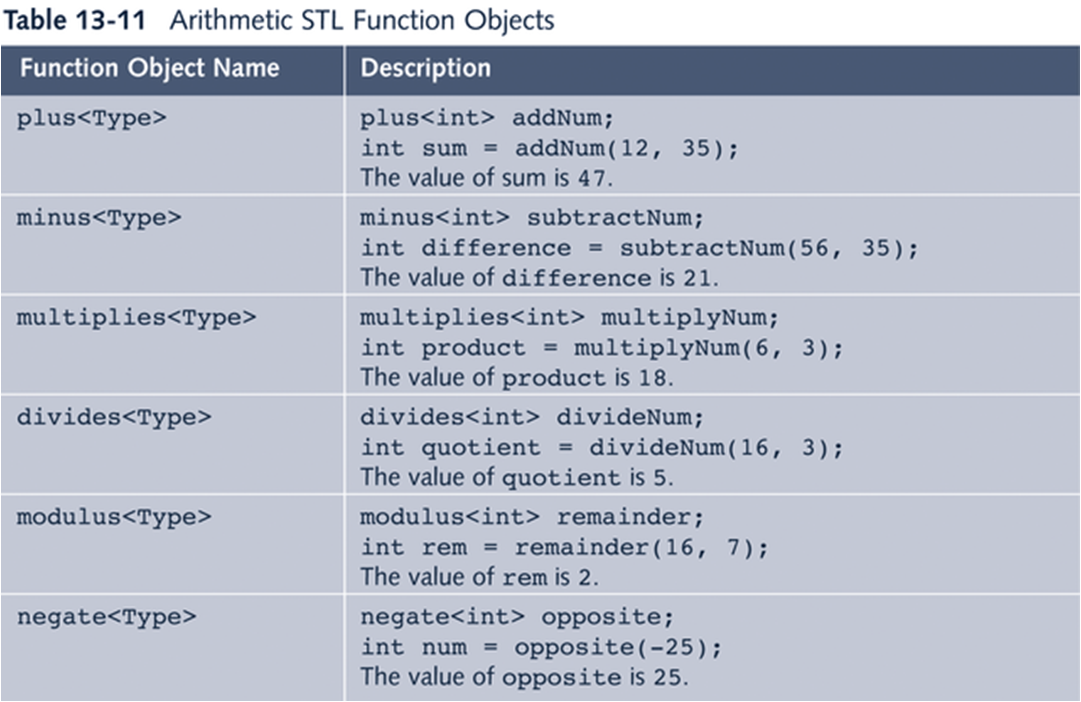
\includegraphics[width=\textwidth]{images/fo1}
\end{center}
\end{frame}

\begin{frame}{Relational STL Function Objects}
\begin{center}
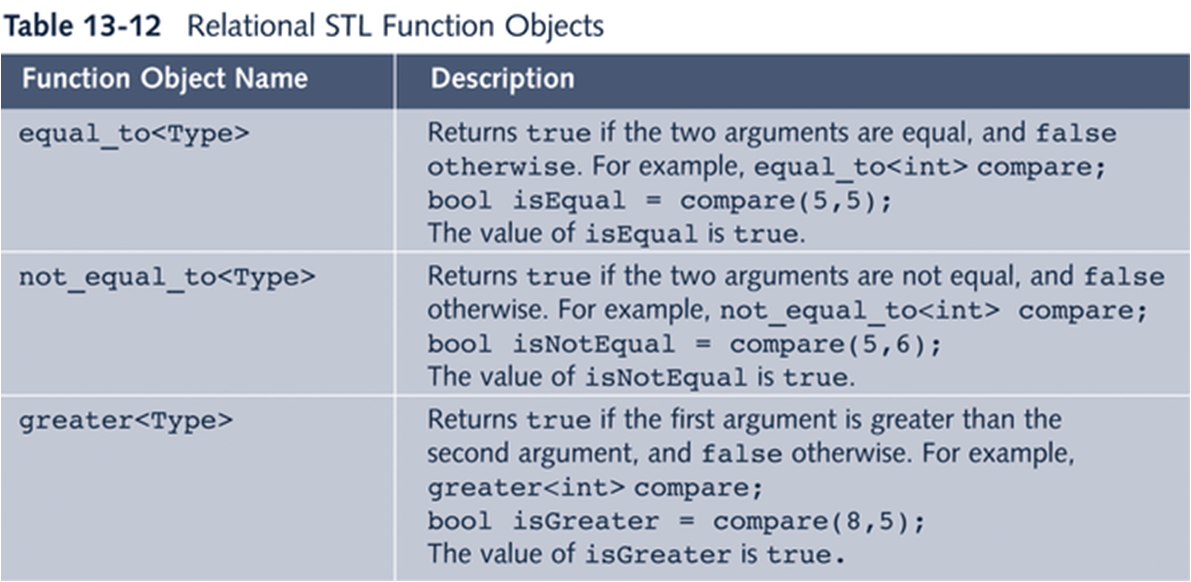
\includegraphics[width=\textwidth]{images/fo2}
\end{center}
\end{frame}

\begin{frame}{Relational STL Function Objects}
\begin{center}
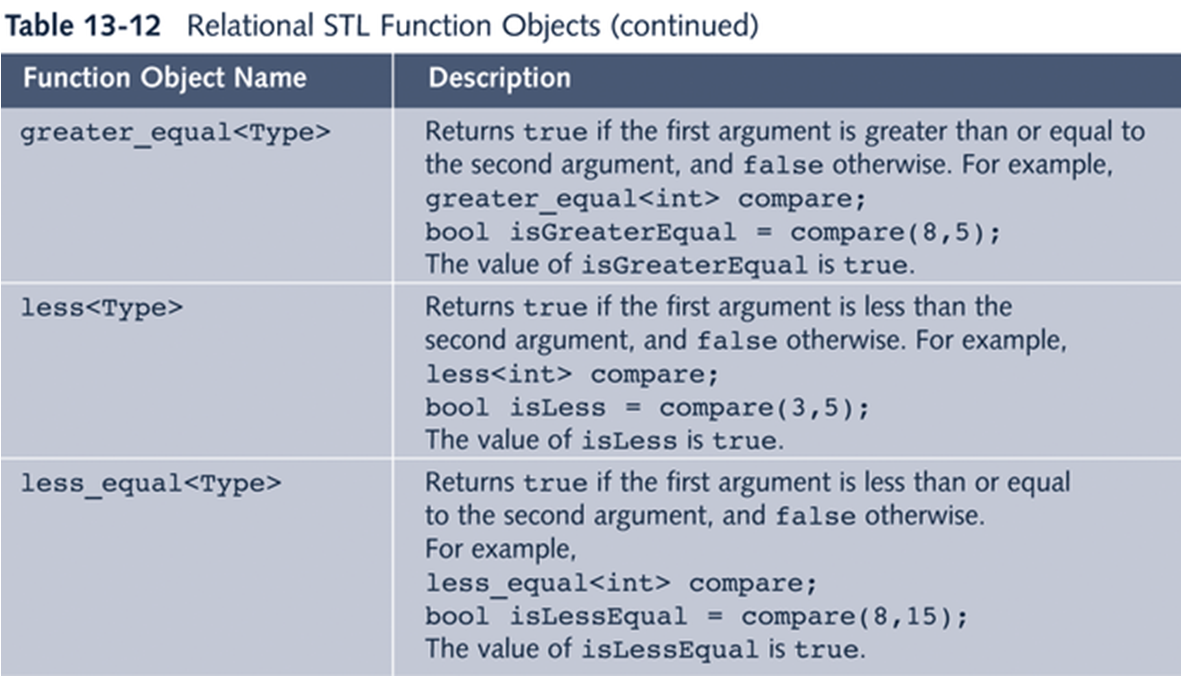
\includegraphics[width=\textwidth]{images/fo3}
\end{center}
\end{frame}

\begin{frame}{Logical STL Function Objects}
\begin{center}
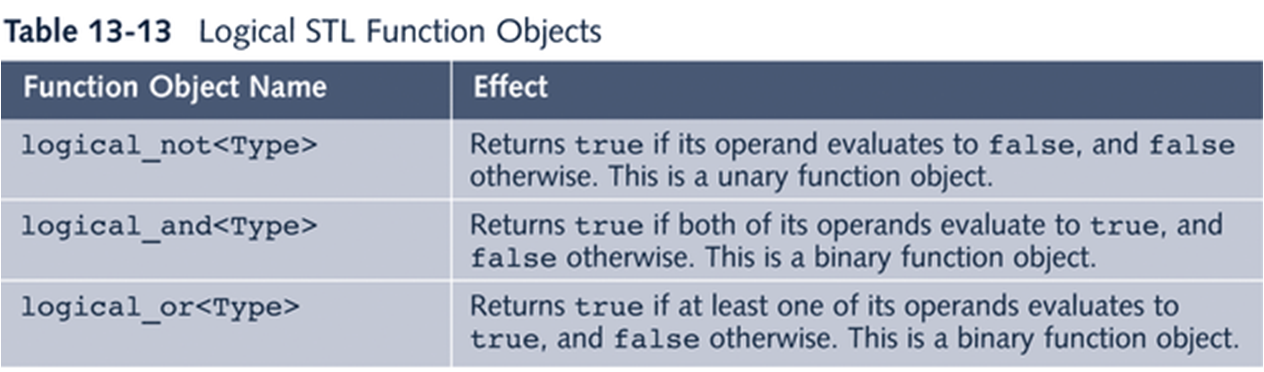
\includegraphics[width=\textwidth]{images/fo4}
\end{center}
\end{frame}

\begin{frame}{Предикати}
\begin{itemize}
  \item Специјален тип на функциски објекти кои враќаат \texttt{boolean} вредност
  \item Унарен предикат, проверува одредено својство на еден елемент 
  \item Бинарни предикати, проверуваат својство за пар  (два аргументи)
  \item Најчесто се користат за да го одредат критериумот при пребарување или
  сортирање
\end{itemize}
\end{frame}
